\documentclass[a4paper,11pt,fleqn]{article}
\usepackage[top=2.5cm,bottom=3cm,right=3cm,left=3cm]{geometry}
\usepackage[utf8]{inputenc}
\usepackage[T1]{fontenc}
\usepackage[french]{babel}
\usepackage{graphicx,graphics,textcomp,setspace,lettrine}
\usepackage{amsmath,amssymb,amsfonts,indentfirst}
\usepackage[toc,page]{appendix} 
\usepackage{float}
\usepackage{array}
\usepackage{comment}
\usepackage{xcolor}
\usepackage{listings}
\usepackage{blindtext}
\usepackage{titling}

\usepackage[english, status=draft]{fixme}
\fxusetheme{color}

\lstset{numbers=left,
numberstyle=\tiny \bf ,
stepnumber=1,
numbersep=10pt,
firstnumber=1,
numberfirstline=true}

\lstset{frame=TBlr,
rulesepcolor=\color{black}}

\DeclareMathOperator{\e}{e}

\usepackage{fancyhdr}
\pagestyle{fancy}

\renewcommand{\headrulewidth}{1pt}
\fancyhead[L]{\leftmark}
\fancyhead[R]{}

\renewcommand{\footrulewidth}{1pt}
\fancyfoot[C]{\textbf{\thepage}} 
\fancyfoot[L]{}

\graphicspath{{results/}}

\title{{\textsc{\Large{Rapport de Méthodologie}\\ [3cm]
      \textbf{\LARGE{Amas de galaxie \\ de Planck}} \\ [0.6cm] 
Etude à travers l'effet \\ Sunyaev-Zel’dovich}} \\[2cm]}
\vfill
\author{Geoffroy Patard De La Vieuville \\ Antoine Marchal}
\date{}


\begin{document}
\begin{titlingpage}
\maketitle
\begin{abstract}
  La collaboration Planck a extrait sur l'ensemble de la mission un
  catalogue d'amas de galaxie (PSZ2) basé sur la détection de l'effect
  Sunyaev-Zel’dovich (SZ). Nous avons, à l'aide de celui-ci,
  reconstruit par ILC (Internal Linear Combination) des estimateurs du
  CMB et de l'effet SZ thermique pour chaque amas. 
  L'étude des poids $w(\nu)$ donnés aux six fréquences des 
  maps de Planck nous apportent une vision sur les différents
  phénomènes physique pouvant intervenir dans l'extraction de ces données. Enfin,
  l'application d'une photométrie d'ouverture nous a ensuite permis 
  d'étudier quelques propriétés de ces amas comme le flux $F=f(z)$ 
  ou encore le rayon critique photométrique $R_{60}=f(z)$.
\end{abstract}
\end{titlingpage}
%\tableofcontents
\thispagestyle{empty}

\newpage

\section{L'effet Sunyaev-Zel’dovich}
L'effet Sunyaev-Zel’dovich est provoqué par la diffusion Compton
Inverse des photons du CMB par le gaz d'électrons chaud ($k_B T_e
\lesssim 15$ KeV) présent dans les amas de galaxies. Son application à
la cosmologie est capitale puisqu'il est de part sa nature
théoriquement indépendant du redshift. Il permet donc l'étude de la
distribution des amas qui est un enjeux important dans la
compréhension du modèle standard de la cosmologie et notamment de la
formation des grandes structures.  

\section{Application de la méthode ILC}
\begin{equation}
  \textbf{w}^t = \frac{\left( \textbf{b}^t\widehat{R}^{-1} \textbf{b}
    \right) \textbf{a}^t \widehat{R}^{-1} - \left( \textbf{a}^t\widehat{R}^{-1} \textbf{b}
    \right) \textbf{b}^t \widehat{R}^{-1}}{\left( \textbf{a}^t\widehat{R}^{-1} \textbf{a}
    \right) \left( \textbf{b}^t\widehat{R}^{-1} \textbf{b}
    \right) - \left( \textbf{a}^t\widehat{R}^{-1} \textbf{b}
    \right)^2}
\end{equation}

\begin{figure}[h]
  \centering
  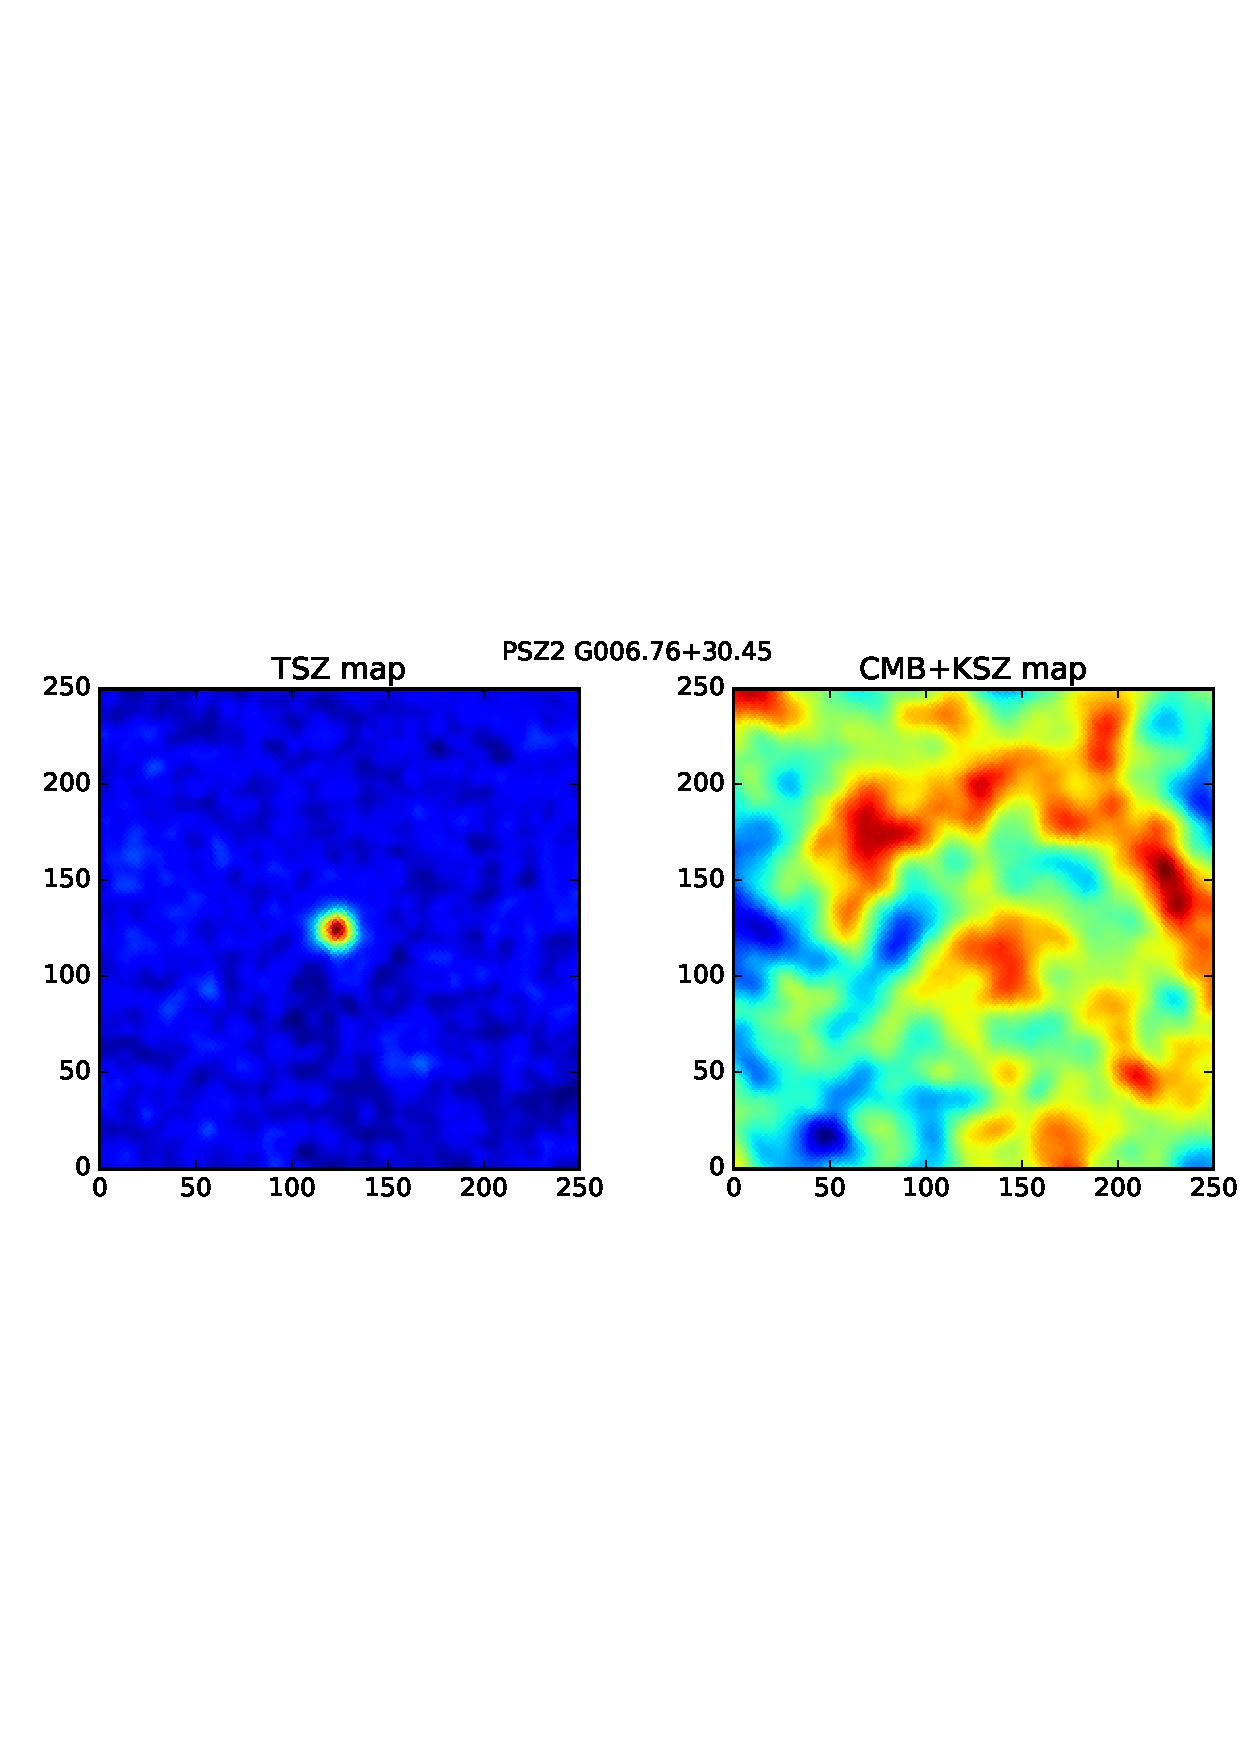
\includegraphics[width=5in]{sz_effect.png}
  \caption{fixme}
\end{figure}
\fxwarning{dimension image sortie python}


\section{Photémétrie d'ouverture}

\section{Résultats et discussion}


\begin{thebibliography}{2}
\addcontentsline{toc}{chapter}{Bibliographie}
   Remazeilles M. \& al., CMB and SZ effect
   separation with Constrained Internal Linear Combinations, 
   Mon. Not. R. Astron. Soc. 410, 2481–2487 (2011) 
\end{thebibliography}
\listoffixmes
\end{document}

